Afin d'étudier la formation planétaire et les interactions avec le disque de gaz, j'ai utilisé un code de simulation N-corps, qui permet de regarder l'évolution d'un nombre arbitraire de corps orbitant autour d'un astre central \citep{chambers1999hybrid}. 

Ce choix est apparu naturellement. Au début de ma thèse, j'ai fait quelques simulations hydrodynamiques avec le code Genesis développé par Arnaud Pierens. J'ai rapidement constaté que ce genre de simulations, bien que modélisant de manière poussée le disque, ne permettait pas d'étudier de manière approfondie la dynamique planétaire. Le temps de calcul nécessaire pour une simulation limite en effet grandement le nombre de corps ainsi que la durée d'intégration. J'ai donc souhaité me tourner vers un code N-corps, afin de privilégier la dynamique planétaire, et de modifier ce programme afin d'y inclure les effets d'un disque de gaz sur la dynamique planétaire. 

J'ai ainsi gagné en temps de calcul, et j'ai ouvert un vaste champ d'investigation sur les paramètres du disque, le nombre de corps en interaction, me permettant de faire des systèmes planétaires très divers, parfois avoir plusieurs centaines d'embryons pour plusieurs millions d'années, chose impossible dans les simulations hydrodynamiques du début de ma thèse où 20 corps pendant quelques dizaines de milliers d'années était un maximum. 

Ce choix a bien entendu introduit son lot d'incertitudes et d'approximations qui sont discutées dans la partie \refsec{sec:discussion}. La présente partie a pour but de présenter le code N-corps que j'ai développé ainsi que les différents effets du disque que j'ai modélisé. J'ai avant tout souhaité présenter les parties qui ont des conséquences sur la physique du disque, que ce soit en terme de choix d'un modèle particulier, ou de limitations numériques qu'il est bien de garder à l'esprit quand on interprète les résultats.

\section{Présentation de Mercury}\index{logiciel!Mercury}
Le code N-corps choisi est le code \textbf{Mercury} \citep{chambers1999hybrid}. Ce code offre la possibilité de choisir un algorithme parmi 5 différents (BS, BS2, RADAU, MVS et HYBRID), ayant des propriétés diverses. Dans le cadre de ma thèse, je n'ai utilisé que l'algorithme HYBRID, qui utilise l'algorithme MVS la plupart du temps, mais change pour l'algorithme BS2 lors de rencontres proches. 

La raison de ce changement est assez simple. MVS est un algorithme symplectique \citep{wisdom1991symplectic}, c'est-à-dire à pas de temps constant, dans lequel on définit un hamiltonien que l'on résout pour faire évoluer les orbites. La conservation de l'énergie est moins bonne que pour un algorithme à pas de temps adaptatif, mais le point très important est que cette conservation de l'énergie se fait sans dérive séculaire. c'est-à-dire que là où les algorithmes tels que BS, BS2 et RADAU verront leur erreur sur l'énergie augmenter au cours du temps, les algorithmes symplectiques vont eux voir leur erreur rester plus ou moins constante au cours du temps. 

Dans le cadre de mes simulations, j'ai accordé une importance limitée aux variations d'énergie, étant donné que les couples que l'on rajoute pour simuler la présence du disque de gaz font que l'énergie n'est pas conservée pour une planète donnée. Cependant, il est important de bien résoudre les orbites et c'est ce point qui est le plus crucial ici. En effet, quelques tests ont permis de contraindre le pas de temps minimal qu'il est nécessaire d'avoir en fonction de la distance orbitale d'une planète. La contrainte de pas de temps dans mes simulations vient donc d'une distance minimale en dessous de laquelle les orbites ne sont pas correctement calculées. Cette limite, afin d'éviter tout problème, est choisie pour être en dessous du bord interne du disque de gaz que je définis.

Les détails techniques et les options de mon code sont détaillés dans l'annexe \refsec{sec:nbody-readme}.

\section{Algorithmes d'intégration}
Dans Mercury, il y a cinq algorithmes différents à notre disposition :
\begin{itemize}
\item MVS \citep{wisdom1991symplectic} : un code symplectique\footnote{Basiquement, un code symplectique est un code qui conserve parfaitement l'énergie de par sa définition en terme d'hamiltoniens.}, c'est-à-dire qui conserve l'énergie au cours du temps et dont le pas de temps est fixe (c'est le seul à avoir un pas de temps fixe)
\item BS \citep{stoer1980introduction} : un algorithme à pas de temps variable, réputé robuste et plutôt long à tourner.
\item BS2 \citep{press1992numerical} : Basé sur BS, il présente l'inconvénient de ne pas fonctionner pour les systèmes non conservatifs. Il est censé être deux fois plus rapide que BS.
\item RADAU \citep{everhart1985efficient} : Ne fonctionne pas bien pour les rencontres proches et les orbites très excentriques. Est censé être deux à trois fois plus rapide que BS.
\item HYBRID \citep{chambers1999hybrid} : Ce code utilise MVS en temps normal, puis lors d'une rencontre proche, utilise BS2 afin de résoudre correctement les orbites.
\end{itemize}

Il y a donc principalement deux catégories : les intégrateurs symplectiques où le paramètre fixe est le pas de temps ($h=\cte$) et les intégrateurs N-corps où le paramètre est la précision en terme de conservation d'énergie d'un pas de temps à l'autre (le pas de temps n'étant pas fixe). Ici, seuls MVS et HYBRID utilisent une partie symplectique alors que BS, BS2 et RADAU sont purement N-corps.

\bigskip

On définit le Hamiltonien $H$ de notre problème N-corps comme étant la somme des énergies cinétiques et potentielles de chaque corps : 
\begin{align}
H &= \sum_{i=1}^N\frac{{p_i}^2}{2m_i} -G\sum_{i=1}^N\sum_{j=i+1}^N\frac{m_im_j}{r_{ij}}
\end{align}
où $m_i$ est la masse du corps $i$, $p_i$ son impulsion et $r_{ij}$ la séparation entre les corps $i$ et $j$.

Un intégrateur symplectique est un intégrateur qui au lieu d'appliquer directement le hamiltonien $H$ sur le système, va séparer ce dernier en deux (ou plusieurs parties) et appliquer ces sous-hamiltoniens successivement. Un intégrateur symplectique résout donc le problème de manière approchée en négligeant les termes croisés des sous-hamiltoniens.

Afin de minimiser l'erreur due à cette approximation, il faut choisir judicieusement la séparation du hamiltonien afin d'avoir une partie dominante par rapport à l'autre.

Par définition, un algorithme symplectique conserve l'énergie au cours du temps, même si l'énergie fluctue au cours du temps autour d'une valeur moyenne. 

Les intégrateurs symplectiques ont deux avantages importants sur les intégrateurs classiques : 
\begin{enumerate}
\item Les fluctuations \og instantanées\fg de l'énergie dues à un algorithme symplectique sont plus grandes que celles d'un
algorithme N-corps, mais à la différence de ces derniers, l'erreur ne croit pas au cours du temps \reffig{fig:energy_error}.
\item Ils sont moins couteux en temps de calcul, en particulier quand la majeure partie de la masse est contenue dans un seul corps (bien adapté pour l'étude d'un système planétaire autour d'une étoile donc).
\end{enumerate}

\begin{figure}[htbp]
\centering
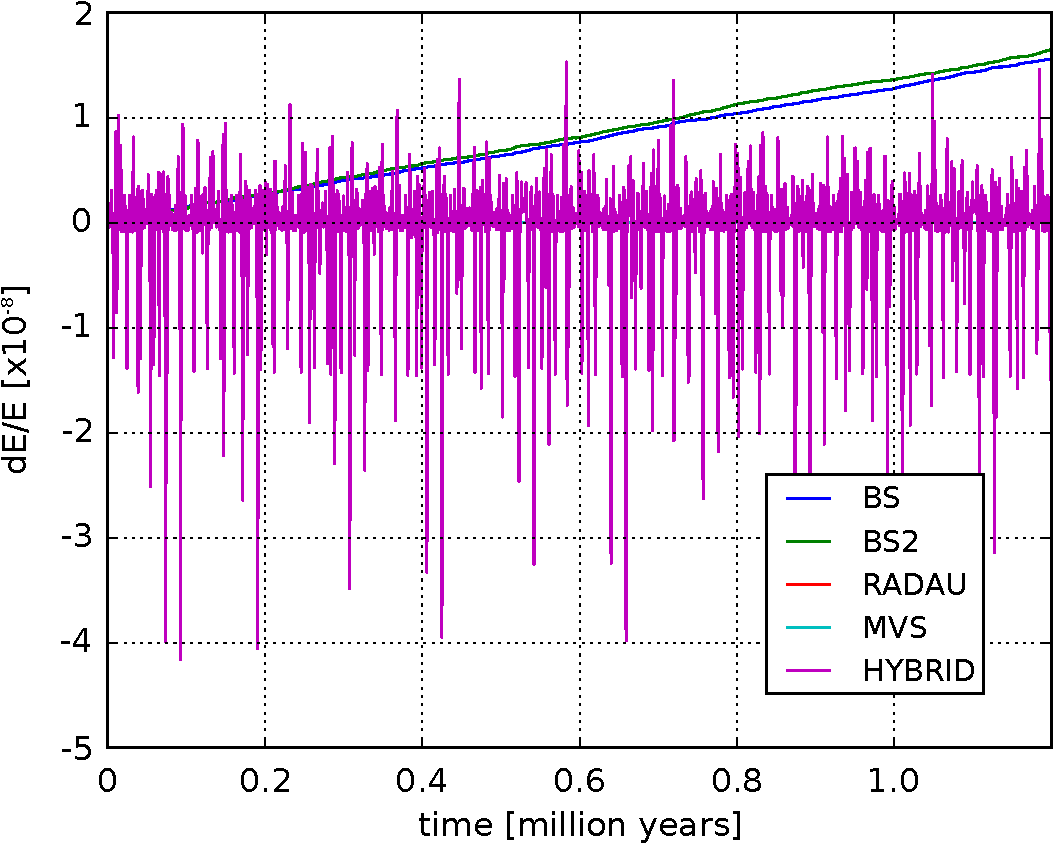
\includegraphics[width=0.65\linewidth]{figure/energy_error.pdf}
\caption[Pour une même simulation, erreur au cours du temps pour BS, BS2, RADAU, MVS et HYBRID.]{Évolution de l'erreur au cours
du temps pour une simulation contenant trois planètes d'une masse terrestre chacune, cette simulation étant lancée
successivement avec chacun des algorithmes disponibles dans \textbf{Mercury}. Les lignes correspondant 
aux intégrateurs MVS et RADAU sont superposées et confondues avec la ligne $\dif E/E=0$.}\label{fig:energy_error}
\end{figure}

Les algorithmes symplectiques ont cependant un inconvénient. Le pas de temps fixe d'un intégrateur symplectique ne permet pas de résoudre correctement les rencontres proches entre les corps du système. Chaque fois que le pas de temps d'un algorithme symplectique est changé, son hamiltonien change aussi, et entraine une variation d'énergie du système (dont l'énergie va osciller autour d'une nouvelle valeur moyenne). 

\bigskip

Nous cherchons maintenant à déterminer l'algorithme le plus approprié pour notre étude. Nous souhaitons faire évoluer un système avec plusieurs dizaines d'embryons planétaires pour plusieurs millions d'années, le système n'étant pas conservatif à cause des divers effets du disque que nous implémentons. 

Nous souhaitons résoudre correctement les orbites, mais avoir un temps de calcul raisonnable. 

La première contrainte est la dissipation. En effet, notre système n'est pas conservatif. Tous les algorithmes N-corps disponibles (BS, BS2 et RADAU) ne fonctionnent donc pas correctement, ces derniers réclament un pas de temps extrêmement faible qui n'est pas représentatif de la précision demandée pour l'intégration N-corps, la variation d'énergie numérique étant masquée par la variation d'énergie induite par les effets du disque. 

Il nous reste les algorithmes MVS et HYBRID. La deuxième contrainte, ce sont les rencontres proches et les collisions. Nous savons qu'un algorithme symplectique ne les traite pas correctement, et si c'est une erreur négligeable dans le cas où il y en a peu, ça ne l'est absolument plus dans notre cas, le nombre de rencontres proches pouvant être très important, notamment dans la phrase d'accrétion en début de simulation. L'algorithme MVS ne parait donc pas adapté contrairement à HYBRID qui a été construit pour être à la fois symplectique et gérer correctement les rencontres proches moyennant une erreur plus importante lors du changement d'algorithme. 

L'algorithme HYBRID est l'algorithme MVS, à pas de temps constant la majorité du temps. Il a donc les avantages d'un algorithme symplectique, à savoir la conservation de l'énergie et la rapidité d'exécution. Lors de rencontres proches (déterminées par une distance minimale d'approche entre deux corps, soit en rayon de Hill, soit en nombre de pas de temps), l'algorithme BS2 est utilisé, le pas de temps devient donc variable afin de résoudre correctement la rencontre et éventuellement la collision. Une fois fini, c'est de nouveau MVS qui prend le relai \citep[voir aussi ][]{mcneil2009new}. 

Dans notre cas, plusieurs approximations sont faites : 
\begin{itemize}
\item L'algorithme BS2 ne fonctionne que pour les systèmes conservatifs. On suppose que la variation d'énergie induite par la migration est totalement négligeable pendant le bref laps de temps de la rencontre proche
\item Le nombre de rencontres proches est suffisamment faible pour que les propriétés symplectiques de l'intégrateur soient 
conservées. On suppose de plus que les variations d'énergies induites par ce biais sont négligeables devant la dissipation 
induite par le disque (qui est de l'ordre de l'énergie initiale du système planétaire)
\end{itemize}

Il reste alors une chose à déterminer, c'est le pas de temps fixe que l'on doit choisir afin de résoudre correctement les orbites. Pour cela, on se place dans un cas simplifié, sans les effets du disque, et on souhaite savoir la condition sur le pas de temps afin que l'orbite soit correctement calculée. 

On ne s'intéresse qu'aux orbites internes qui sont limitantes au niveau du pas de temps en raison de leur période réduite. Pour une planète à une distance de $0.1\unit{UA}$ du soleil, la période orbitale est de 11 jours environ.

On réalise deux tests. Dans le premier test, on fait évoluer une planète de $1\mearth$ totalement isolée. On fait varier son demi-grand axe et son excentricité et on regarde comment évolue la conservation de l'énergie. Étant donné qu'avec un algorithme symplectique l'énergie oscille au cours du temps, on prend la valeur moyenne de la variation d'énergie, moyenne effectuée sur une centaine de valeurs.

Dans un deuxième test, on procède exactement de la même manière, à ceci près qu'on place une planète de $1\unit{M_\text{jup}}$ à $5\unit{UA}$. 

\reffig{fig:accuracy_maps} montre l'évolution de la conservation de l'énergie dans ces deux tests pour deux pas de temps différents, $h=1\unit{jour}$ et $h=0.4\unit{jour}$. Pour un pas de temps donné, nous ne pouvons pas donner simplement de position en dessous de laquelle l'orbite n'est pas correctement résolue. L'excentricité a une influence. En effet, la distance minimale entre l'étoile et la planète se situe au périhélie, mais suivant l'excentricité, la planète passera plus ou moins de temps au périastre. Ainsi, une très grande excentricité va diminuer drastiquement le temps passé au périastre, pour un périastre donné \citep{rauch1999dynamical, levison2000symplectically}. 

\begin{figure}[htbp]
\centering
\subfloat[$h=1\unit{jour}$ sans Jupiter]{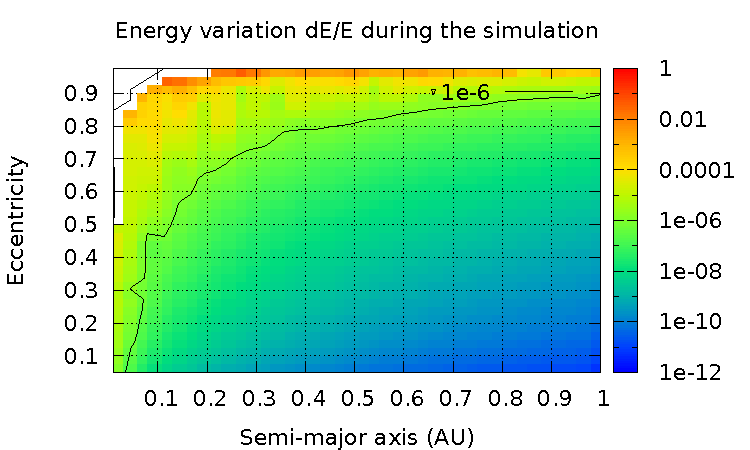
\includegraphics[width=0.49\textwidth]{figure/accuracy_10_one.pdf}}\hfill
\subfloat[$h=1\unit{jour}$ avec Jupiter]{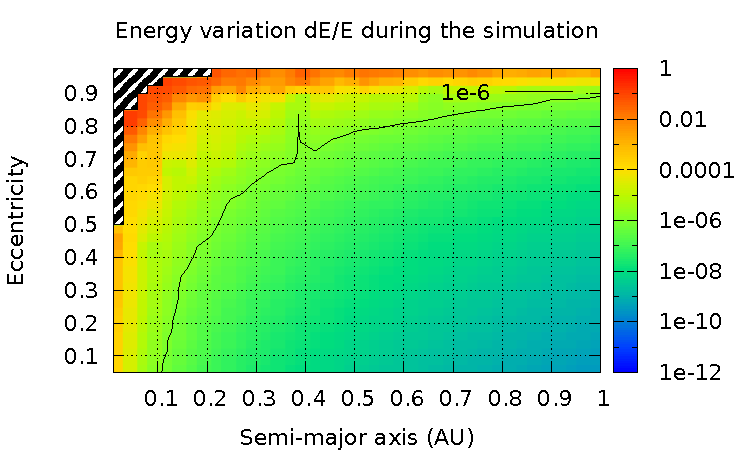
\includegraphics[width=0.49\textwidth]{%
figure/accuracy_10_jup.pdf}}

\subfloat[$h=0.4\unit{jour}$ sans Jupiter]{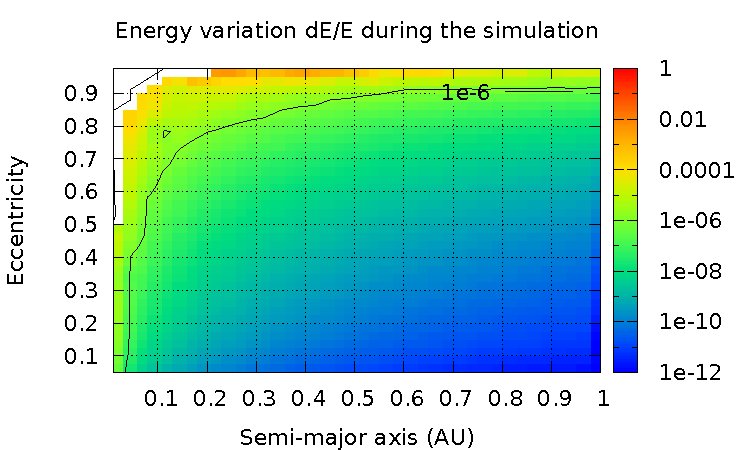
\includegraphics[width=0.49\textwidth]{figure/accuracy_04_one.pdf}}\hfill
\subfloat[$h=0.4\unit{jour}$ avec Jupiter]{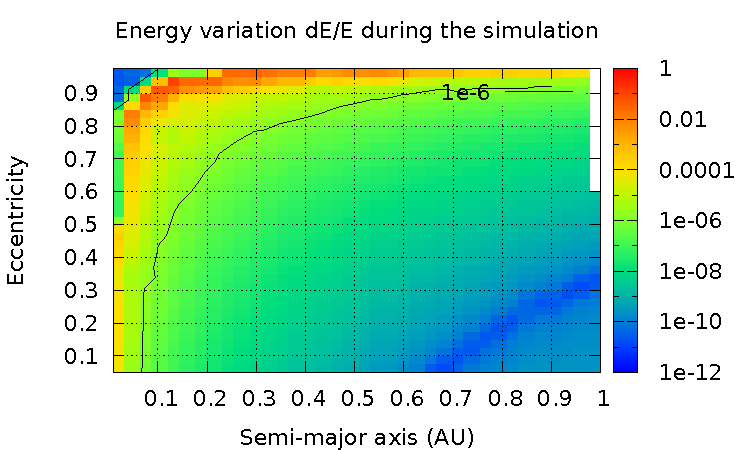
\includegraphics[width=0.49\textwidth]{%
figure/accuracy_04_jup.pdf}}


\caption[Conservation de l'énergie en fonction du pas de temps et des conditions initiales.]{Tests pour $h=1\unit{jour}$ et
$h=0.4\unit{jour}$ de la conservation de l'énergie pour une planète de $1\mearth$ isolée ou avec un compagnon de la taille de
Jupiter. Les cartes montrent la conservation de l'énergie pour différentes valeurs du demi-grand axe $a$ et de l'excentricité
$e$. La ligne noire correspond à un $\dif E/E=10^{-6}$, valeur en dessous de laquelle on considère que la précision sur l'orbite
est suffisante. La partie hachurée correspond à la collision de la planète interne avec l'étoile centrale donc le rayon est
$R_\star=0.005\unit{UA}$.}\label{fig:accuracy_maps}
\end{figure}

Si un pas de temps plus grand ($h=1\unit{jour}$) semble convenir pour une planète isolée, la conservation de l'énergie est
différente dans le cas avec des perturbations gravitationnelles (cas avec Jupiter). À $0.1\unit{UA}$, qui correspond au bord
interne, zone particulièrement importante pour notre étude, ce pas de temps ne convient plus. Dès que l'excentricité augmente un
peu, la précision sur l'orbite diminue, et les orbites les plus internes ne sont pas correctement résolues.

Même si le disque amortit les excentricités, nous souhaitons résoudre correctement les orbites légèrement excentriques, même au bord interne à $0.1\unit{UA}$. Un pas de temps de $h=1\unit{jour}$ résout correctement les orbites au bord interne, même légèrement excentriques, mais uniquement dans le cas d'une planète isolée. Si on ajoute les perturbations d'une planète externe, les orbites au bord interne ne sont plus correctement résolues. Ce défaut est corrigé si nous prenons un pas de temps de $h=0.4\unit{jour}$. C'est donc celui que nous utiliserons par défaut.

Un moyen mnémotechnique pour calculer le pas de temps minimal pour une simulation est de considérer qu'il faut résoudre l'orbite la plus proche avec un minimum de $10$ pas de temps. Ceci n'est valable que dans l'approximation où l'excentricité n'est pas trop élevée ($e<0.4$). Si nous faisons ce calcul ici, nous obtenons qu'avec un demi-grand axe minimal de $a=0.1\unit{UA}$ et une excentricité maximale de $e=0.4$, la distance minimale d'approche est $q=0.06$. La période d'une orbite $a=0.06$ est de $5\unit{jours}$ environ, ce qui donne un pas de temps maximal de $h=0.5\unit{jour}$. 

\section{Disque (1+1)D}
Afin de calculer les effets d'un disque de gaz, une modélisation de ce dernier est nécessaire. Le but étant d'avoir une grande
souplesse, le disque implémenté est bien entendu très simplifié. Toutes les quantités sont intégrées selon la hauteur $z$ et la
position azimutale $\theta$ dans le disque, résultant en un modèle radial 1D de toutes les quantités. Le nombre de points de
tous les profils est identique pour une même simulation. Typiquement le nombre de points égal à $n=1000$. Les points ne sont
pas régulièrement espacés, le nombre est plus important au bord interne de sorte que l'espacement $\Delta X$ entre les points
est constant, où $X$ est défini comme : 
\begin{align}
X = \log{R}
\end{align}

Dans la mesure du possible, les quantités du disque ont été calculées de manière cohérente. Je vais présenter dans la suite de manière chronologique comment sont calculées les grandeurs physiques du disque.

\subsection{Profil de densité de surface}
Le profil de densité de surface est défini au début de la simulation comme une loi de puissance de la forme :
\begin{align}
\Sigma(R) &= \Sigma_0 \times R^{-d}
\end{align}
où $\Sigma_0$ est la densité de surface à $1\unit{UA}$ et $d$ l'indice de la loi de puissance. 

Ce profil de densité de surface est défini pour une certaine étendue radiale. On définit donc un bord interne $R_\text{in}$ et un bord externe $R_\text{out}$. Le bord interne est généralement à $0.1\unit{UA}$ et le bord externe à $100\unit{UA}$. 

Afin de calculer les valeurs suivantes, ce disque est échantillonné et toutes les valeurs nécessaires sont ensuite calculées à chacun de ces points. 

\bigskip

Le profil de densité de surface est le paramètre d'entrée le plus important. Il est celui à partir duquel on calcule toutes les autres quantités du disque, température, échelle de hauteur, etc\dots

Le profil étant une loi de puissance, un amortissement est effectué au bord interne du disque afin que la valeur de la densité au bord interne soit proche de zéro. 

Le profil de densité de notre disque de référence (dont nous parlerons plus en détail \refsec{sec:migrations-maps}) est représenté \reffig{fig:fiducial_density}

\begin{figure}[htbp]
\centering
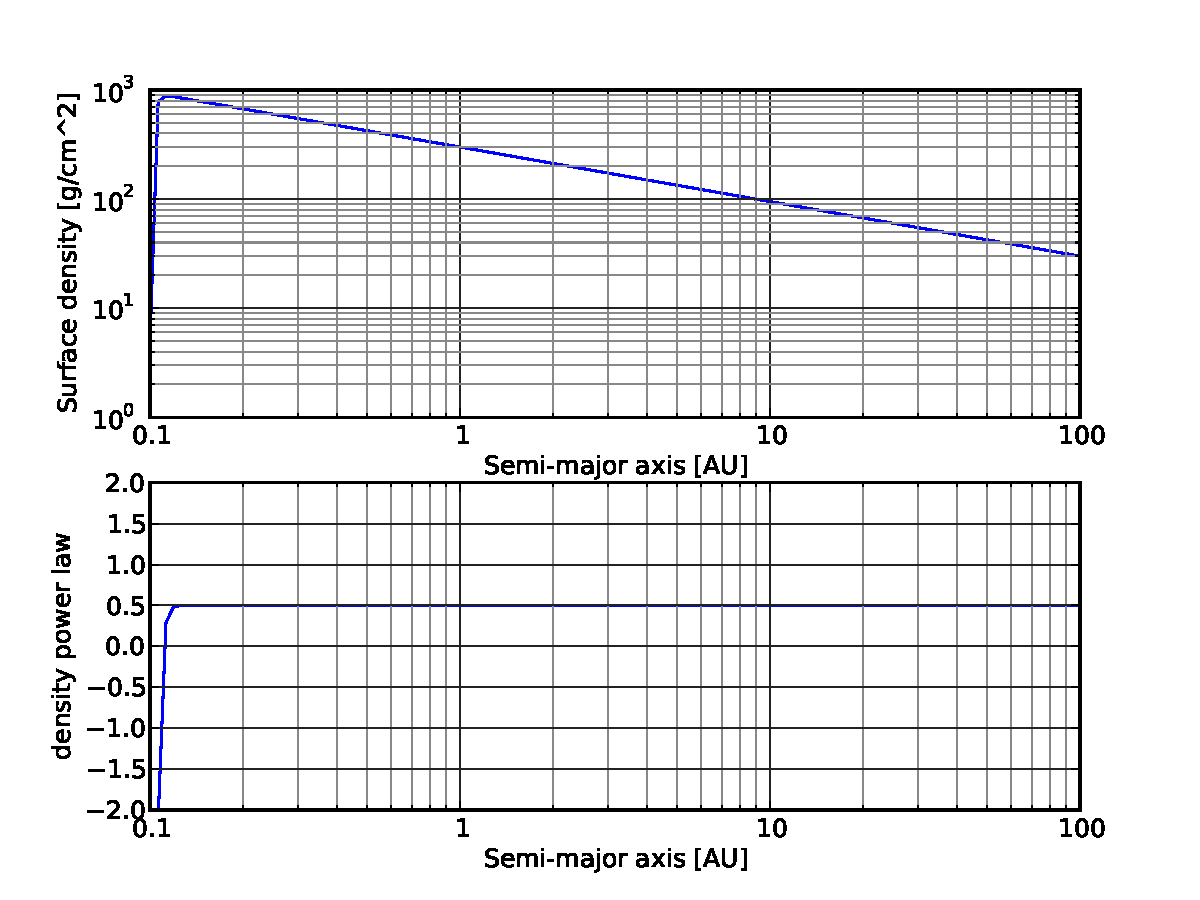
\includegraphics[width=0.75\linewidth]{figure/fiducial_density_profile.pdf}
\caption{Profil de densité de surface pour notre disque de référence \protect\reftab{tab:fiducial_parameters}.}\label{fig:fiducial_density}
\end{figure}

\subsection{Table d'opacité}\index{opacité}
Afin de pouvoir calculer le profil de température, on a besoin de choisir un modèle pour l'opacité. Je ne détaillerai pas ici les différents modèles car une étude spécifique a été menée \refsec{sec:influence_opacity_table} afin de comprendre l'influence du choix du modèle sur les résultats des simulations. 

Par contre, quel que soit le modèle, on a généralement une dépendance en fonction de la densité et de la température. L'opacité est donc un paramètre de la résolution de l'équation qui nous permet d'avoir la température. L'opacité n'est pas, dans notre modèle, une quantité qu'on fixe \emph{a priori}, mais plutôt un des paramètres de sortie de la résolution de l'équation de l'énergie dans le disque.

\subsection{Profil de température}
Afin de construire le profil de température point par point, on résout, pour chaque position dans le disque définie dans le profil, l'équation de l'énergie \refeq{eq:equation_energie}. 

De manière consistante, cette équation a pour paramètre d'entrée la position, et on cherche à trouver les valeurs de la température $T$, échelle de hauteur $H$, profondeur optique $\tau$, diffusivité thermique $\chi$. Toutes ces valeurs sont fixées une fois qu'un ensemble cohérent de valeurs satisfont l'équation.

Afin de résoudre cette équation du type $f(x)=0$, j'ai utilisé une version modifiée de la routine \textbf{zbrent} de \textbf{Numerical Recipes} \citep{press1992numerical}. Cette routine utilise la méthode de Van Wijngaarden-Dekker-Brent. Cette méthode est une combinaison de plusieurs méthodes et permet d'assurer la convergence tout en étant relativement rapide.

Le profil de température que nous obtenons dans notre disque de référence (dont nous parlerons plus en détail \refsec{sec:migrations-maps}) est représenté \reffig{fig:fiducial_temperature}

\begin{figure}[htbp]
\centering
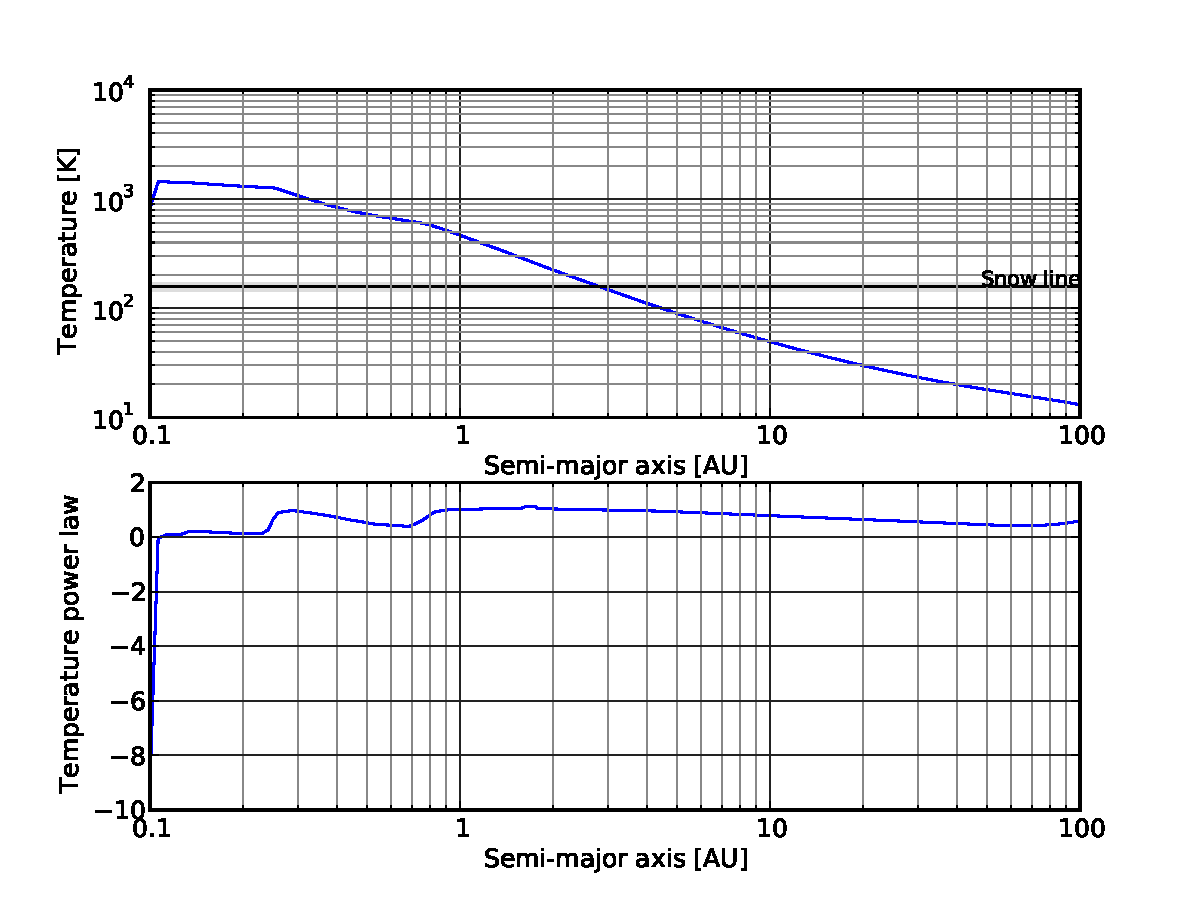
\includegraphics[width=0.75\linewidth]{figure/fiducial_temperature_profile.pdf}
\caption{Profil de température pour notre disque de référence \protect\reftab{tab:fiducial_parameters}.}\label{fig:fiducial_temperature}
\end{figure}

\section{Migration de Type I}\index{migration!Type I}
La migration de Type I est implémentée dans le code en utilisant le modèle 1D de disque, qui définit pour toute position du 
disque, une température, une densité de surface, et tous les autres paramètres nécessaires comme l'échelle de hauteur. En 
utilisant ces paramètres, on obtient ainsi le couple qu'exerce le disque sur la planète en fonction de sa masse et de sa 
position via la formule semi-analytique de \cite{paardekooper2011torque}. Plus exactement, j'implémente les formules décrites 
\refsec{sec:type_I}, équations \refeq{eq:lindblad-torque}, \refeq{eq:saturated-corotation-torque} et 
\refeq{eq:linear-corotation-torque}. Ces formules sont une combinaison de \cite{paardekooper2010torque} où l'effet du paramètre 
de lissage $b/h$ apparaît de manière explicite, mais qui ne modélise que les couples linéaires, et \cite{paardekooper2011torque} 
où l'effet de la diffusion est pris en compte, mais où la longueur de lissage n'apparait pas explicitement. Ainsi, nous 
obtenons des formules pour la migration de Type I qui dépendent du paramètre de lissage $b/h$(\refeq{eq:lindblad-torque}, 
\refeq{eq:saturated-corotation-torque} et 
\refeq{eq:linear-corotation-torque}), et qui en plus tiennent compte 
de la saturation \citep[eqs. (50) à (53)]{paardekooper2011torque}.

Les deux différences principales entre le cadre du modèle de \cite{paardekooper2011torque} et le disque que j'ai modélisé, c'est que dans mon cas je n'ai pas un profil de température en loi de puissance (avec une seule loi de puissance), mais j'ai une loi de puissance définie point par point. C'est-à-dire que pour chaque zone du disque, la température est calculée de manière cohérente avec les autres paramètres du disque, et que l'indice de la loi de puissance correspondante est calculée en fonction des températures autour.

La deuxième différence est que j'ai un profil pour l'échelle de hauteur $H$ et le rapport d'aspect $h=H/R$ du disque au lieu d'avoir un rapport d'aspect constant pour tout le disque.

\bigskip

De plus, certaines erreurs se sont glissées dans ce papier. \cite[appendice A]{bitsch2011range} fait remarquer en particulier qu'il manque un facteur 4 dans l'équation (33). Ainsi, la formule que j'ai utilisé pour calculer la conductivité thermique $\chi$ est :
\begin{align}
\chi &= \frac{16\gamma (\gamma-1) \sigma T^4}{3\kappa \rho^2 H^2\Omega^2}
\end{align}

Il y a aussi une erreur dans l'équation (35) car le disque se refroidit par la surface supérieure et la surface inférieure. Mais comme j'utilise dans mon code une équation de l'énergie \refeq{eq:equation_energie} un peu plus complexe où j'ai tenu compte de ce fait là, cette erreur n'a pas d'incidence sur le calcul du couple.

Les formules nous donnent alors un couple exercé par le disque sur la planète. 

À partir de ce couple, on définit un temps de migration $t_\text{mig}=r_p / (-\dot{r}_p)$ comme \citep[eq. 
(69)]{tanaka2002three}: 
\begin{align}
t_\text{mig} &= -\frac{J}{2\Gamma}
\end{align}
où $J$ est le moment cinétique total de la planète et $\Gamma=\dot{J}$ est le couple total exercé par le disque sur la planète.

\bigskip

On cherche maintenant à trouver une expression de l'accélération spécifique due à la migration $\vect{a_\text{mig}}$ qui va être sous la forme : 
\begin{align*}
\vect{a_\text{mig}} &= -\frac{\vect{v}}{\tau}
\end{align*}
où $\tau$ est le facteur que l'on cherche.

On écrit alors la somme des forces par unité de masse : 
\begin{align*}
\vect{a} &= \vect{F_g} + \vect{F_\text{mig}}\\
\vect{a} &= -\frac{GM}{r^2}\hat{e}_r - \frac{\vect{v}}{\tau}
\end{align*}
On projette cette équation en coordonnées cylindriques (ce qui revient à décomposer la vitesse et l'accélération en cylindrique) :
\begin{subequations}
\begin{align}
\ddot{r} - r\dot{\theta}^2 &= -\frac{GM}{r^2} -\frac{\dot{r}}{\tau}\\
r\ddot{\theta} + 2 \dot{r}\dot{\theta} &= - \frac{r\dot{\theta}}{\tau}\label{eq:mig_proj_theta}
\end{align}
\end{subequations}

Le moment cinétique vaut : 
\begin{align*}
\vect{J} &= \vect{r} \wedge \vect{v} = r \hat{e}_r \wedge \left( \dot{r}\hat{e}_r + r\dot{\theta}\hat{e}_\theta\right)\nonumber\\
\vect{J} &= r^2\dot{\theta}\hat{e}_z
\end{align*}

La dérivée de la norme du moment cinétique vaut :
\begin{align*}
\od{\norm{\vect{J}}}{t} &= r\ddot{\theta} + 2 \dot{r}\dot{\theta}
\end{align*}

On fait apparaître la norme du moment cinétique et de sa dérivée dans \refeq{eq:mig_proj_theta} en multipliant tout par $r$ : 
\begin{align*}
\dot{J} &= - \frac{J}{\tau}\nonumber\\
\tau &= - \frac{J}{\dot{J}}
\end{align*}
On utilise alors la définition de $t_\text{mig}$ pour obtenir :
\begin{align*}
\tau &= 2 t_\text{mig}
\end{align*}

On a ainsi
\begin{important}
\begin{align}
\vect{a_\text{mig}} &= -\frac{\vect{v}}{2 t_\text{mig}}
\end{align}
\end{important}
où $\vect{v}$ est la vitesse instantanée de la planète.

\section{Amortissement de e et I}
L'amortissement de l'excentricité $e$ et de l'inclinaison $I$ d'une planète plongée dans un disque protoplanétaire est modélisé
dans le code via les formules de \cite[eq. (9), (11) et (12)]{cresswell2008three} : 
\begin{subequations}
\begin{align}
t_e &= \frac{t_\text{wave}}{0.780}\left[1-0.14\left(\frac{e}{H/r}\right)^2 + 0.06 \left(\frac{e}{H/r}\right)^3 + 0.18\left(\frac{e}{H/r}\right)\left(\frac{I}{H/r}\right)^2\right]\\
t_I &= \frac{t_\text{wave}}{0.544}\left[1-0.30\left(\frac{I}{H/r}\right)^2 + 0.24 \left(\frac{I}{H/r}\right)^3 + 0.14\left(\frac{e}{H/r}\right)^2\left(\frac{I}{H/r}\right)\right]\\
t_\text{wave} &= \frac{M_\star}{m_p}\frac{M_\star}{\Sigma_p {a_p}^2}\left(\frac{H}{r}\right)^4{\Omega_p}^{-1}
\end{align}
\end{subequations}

Les accélérations spécifiques dues à l'excentricité  et l'inclinaison sont définies par \citep[eq. (15) et (16)]{cresswell2008three} : 
\begin{subequations}
\begin{align}
\vect{a_e} &= -2 \frac{(\vect{v}.\vect{r})}{r^2 t_e}\vect{r}\\
\vect{a_i} &= - \frac{\vect{v_z}}{t_i}\hat{e}_z
\end{align}
\end{subequations}

L'amortissement de $I$ est arrêté quand l'inclinaison descend en dessous de $I<5\cdot 10^{-4}\unit{rad}$ afin d'empêcher les planètes d'être parfaitement dans le plan $(x,y)$, essentiellement pour empêcher des problèmes numériques.

\section{Effet de l'excentricité sur le couple de corotation}\index{amortissement!couple de corotation}
Afin de tenir compte d'un effet mis en évidence par \cite{bitsch2010orbital}, une petite modification a été effectuée dans le calcul du couple total $\Gamma$ exercé par le disque sur la planète. 

En effet, il a été montré que l'excentricité d'une planète a une influence sur sa zone fer-à-cheval et par extension, sur son couple de corotation $\Gamma_C$. Un paramètre d'amortissement $D$, compris entre 0 et 1 a ainsi été ajouté au calcul du couple total \citep{hellary2012global} :
\begin{align}
\Gamma &= \Gamma_0 \cdot (\frac{\Gamma_L}{\Gamma_0} + D\cdot \frac{\Gamma_C}{\Gamma_0})
\end{align}
où $\Gamma_0 = \left(\frac{q}{h}\right)^2\Sigma_p {r_p}^4 {\Omega_p}^2$ et $\Gamma_L$ est le couple de Lindblad.

La valeur du paramètre d'amortissement $D$ est donnée par une formule qui a été calculée pour coller au mieux aux simulations de \cite{bitsch2010orbital}, détaillée dans \cite{cossou2013convergence}, et recopiée ici : 
\begin{subequations}
\begin{align}
D = \frac{\Gamma_C(e)}{\Gamma_C (e=0)} &= 1 + a \cdot \left[\tanh(c) - \tanh\left(\frac{b * e}{x_s}+c\right)\right]\label{eq:eccentricity-influence}\\
a &= 0.45 \qquad b=3.46 \qquad c= -2.34
\end{align}
\end{subequations}
où $x_s$ représente la demi-largeur de la région fer-à-cheval adimensionnée.

\section{Désactivation des effets du disque}
Quand une planète sort des bornes du disque, les effets d'amortissement de $e$ et $I$ sont désactivés, au même titre que la migration due à la présence du disque. Ce cas survient rarement au bord externe du disque (généralement à $100\unit{UA}$), mais est beaucoup plus probable au bord interne (généralement à $0.1\unit{UA}$).

\section{Validité des éléments orbitaux}
Lors d'une rencontre proche entre deux planètes, leurs interactions gravitationnelles rendent caduques les formules qui permettent de calculer les éléments orbitaux à partir des vitesses et positions car ceci suppose qu'on est dans le cas d'une orbite képlerienne isolée. 

Dans de tels cas, on peut avoir des demi-grands axes négatifs, des excentricités supérieures à 1. Si c'est déjà en soit un 
problème physique, c'est aussi et surtout un problème numérique car cela fait apparaître des \textbf{Not A Number} (NaN) lorsque 
par exemple le demi-grand axe est en argument d'une racine carrée. Ceci a donc pour conséquence concrète de faire planter le 
code, au mieux, ou pire, de le faire tourner avec tous les paramètres de la simulation peu à peu gangrénés par des 
\textbf{NaN}. 

Dans un premier temps, j'ai pensé remplacer dans mes calculs le demi-grand axe par le rayon $r=\sqrt{x^2+y^2+z^2}$, afin 
d'éviter les problèmes lors des rencontres proches. Cette solution fait apparaître d'autres problèmes, notamment avec des 
orbites excentriques proches du bord interne. Dans ce cas, on peut avoir une planète qui ressent un couple positif au bord 
interne, puis plus de couple du tout dans la partie de l'orbite qui sort du disque, et enfin un couple négatif quand la planète 
est dans le disque, mais hors du bord interne. Ceci cause de gros problèmes et génère des orbites qui ne sont pas physiques 
mais dues à une astuce qui cherche à contourner un problème numérique. En effet, les formules de migration sont moyennées sur 
une orbite, on ne peut donc pas avoir de telles variations au sein d'une même orbite.

La solution adoptée est de tester les cas qui causent des NaN, c'est à dire typiquement des excentricités supérieures à 1, et 
un demi-grand axe négatif. Quand de tels cas surviennent, on désactive momentanément la migration et tous les effets du 
disque. Le reste du temps, la migration est systématiquement calculée, y compris pendant les rencontres proches. On considère 
que le temps durant lequel le calcul des éléments orbitaux n'est plus valide représente un temps négligeable de la 
simulation au regard des centaines de milliers d'années sur lesquelles on intègre les orbites. On considère donc que la 
migration induite sur les planètes pendant les rencontres proches est totalement négligeable au regard du reste de la 
simulation.
